% ============================================================================
% Chapter 4: Electrical System Architecture and Embedded Design
% ============================================================================

\chapter{Electrical System Architecture and Embedded Design}
\label{chap:electrical}

\section{Overview}
\label{sec:electrical_overview}

This chapter details the design, implementation, and integration of the electrical subsystems for the AUSRA mobile robot platform. The electrical architecture is designed to support a robust, autonomous swarm capability by prioritizing three key engineering principles:

\begin{enumerate}
    \item \textbf{Hierarchical Control:} Decoupling high-level AI processing from low-level real-time actuation ensures that computationally intensive tasks such as SLAM and path planning do not interfere with time-critical motor control loops.
    \item \textbf{Power Isolation:} Separating noisy motor loads from sensitive logic circuits prevents electromagnetic interference and voltage fluctuations from corrupting sensor data or causing computational errors.
    \item \textbf{Modular Safety:} Implementing physical hardware failsafes for charging and operation protects both the user and the electronic components from hazardous conditions.
\end{enumerate}

\section{System Topology}
\label{sec:system_topology}

The system is built upon a distributed power and control architecture. A central 20V DC bus, derived from a high-discharge Lithium-Ion source, powers two distinct regulation stages: the \textbf{Logic Stage} for computation and sensors, and the \textbf{Actuation Stage} for motor propulsion.

The control hierarchy consists of an NVIDIA Jetson Orin Nano serving as the high-level ``Brain'' (handling SLAM, path planning, and vision), which communicates via serial interface with an ESP32 Microcontroller, acting as the low-level ``Spine'' (handling inverse kinematics, PID control, and IMU data acquisition).

\begin{figure}[H]
    \centering
    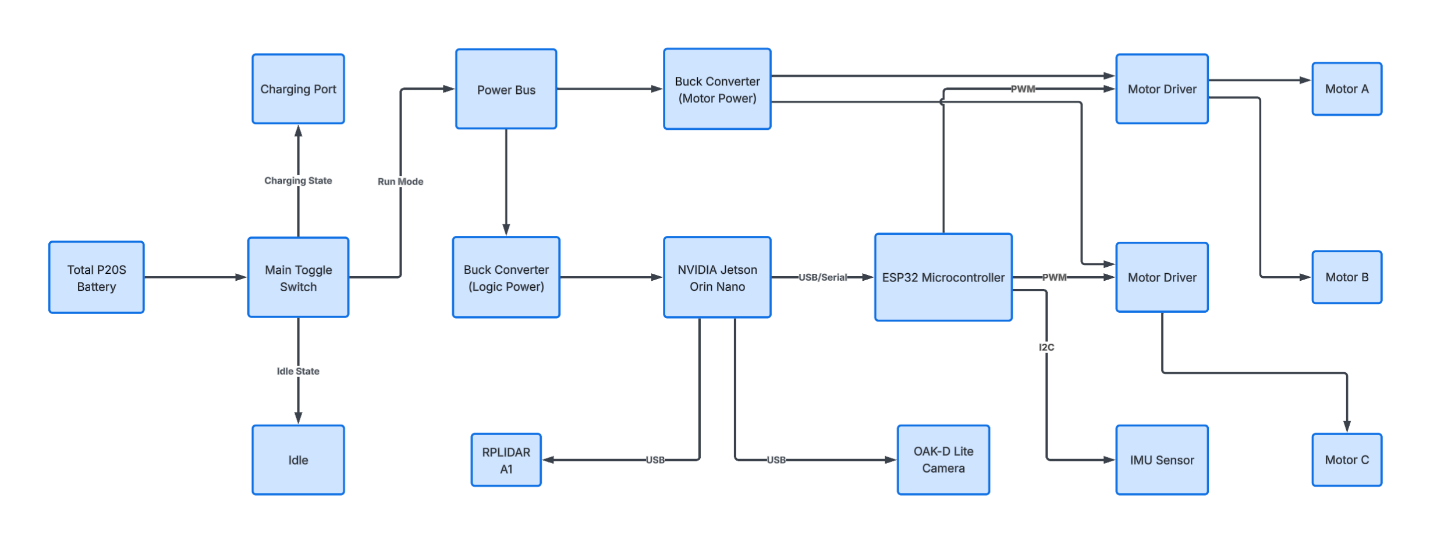
\includegraphics[width=0.85\linewidth]{figures/Chapter 4/System_topology.png}
    \caption{Electrical System Topology showing the hierarchical control architecture}
    \label{fig:system_topology}
\end{figure}

\section{Component Selection and Justification}
\label{sec:component_selection}

The selection of hardware components was driven by the specific requirements of holonomic motion and edge-AI processing. Each component underwent rigorous evaluation using weighted decision matrices to ensure optimal performance within the project constraints.

\subsection{Low-Level Controller Selection}
\label{subsec:lowlevel_controller}

The selection of the low-level microcontroller was critical for ensuring reliable real-time motor control and seamless communication with the high-level ROS 2 stack. Three candidates were evaluated: \textbf{Teensy 4.1}, \textbf{STM32F411}, and \textbf{ESP32-S3}.

\subsubsection{Selection Criteria}

\begin{enumerate}
    \item \textbf{Micro-ROS Compatibility:} The ability to run micro-ROS agents natively for seamless node integration with the ROS 2 ecosystem \cite{microros2023}.
    \item \textbf{Ease of Development:} The learning curve required to implement drivers; specifically comparing the Arduino ecosystem against vendor-specific HALs (Hardware Abstraction Layers).
    \item \textbf{Memory \& Performance:} SRAM size for buffering ROS messages and clock speed for executing PID loops at high frequency.
    \item \textbf{Cost:} Unit cost per board, which scales significantly across a swarm deployment.
\end{enumerate}

\subsubsection{Selection Matrix}

\begin{table}[H]
\centering
\caption{Microcontroller Weighted Decision Matrix (Scale: 1 = Poor, 10 = Excellent)}
\label{tab:mcu_selection}
\begin{tabular}{|l|c|c|c|c|}
\hline
\textbf{Criteria} & \textbf{Weight} & \textbf{Teensy 4.1} & \textbf{STM32F411} & \textbf{ESP32-S3} \\ \hline
Micro-ROS Support & 0.30 & 8 & 6 & 10 \\ \hline
Ease of Use & 0.25 & 10 & 5 & 9 \\ \hline
Memory / Specs & 0.25 & 10 & 6 & 7 \\ \hline
Cost Efficiency & 0.20 & 3 & 10 & 9 \\ \hline
\textbf{Weighted Score} & \textbf{1.00} & \textbf{7.95} & \textbf{6.55} & \textbf{8.80} \\ \hline
\end{tabular}
\end{table}

\begin{figure}[H]
    \centering
    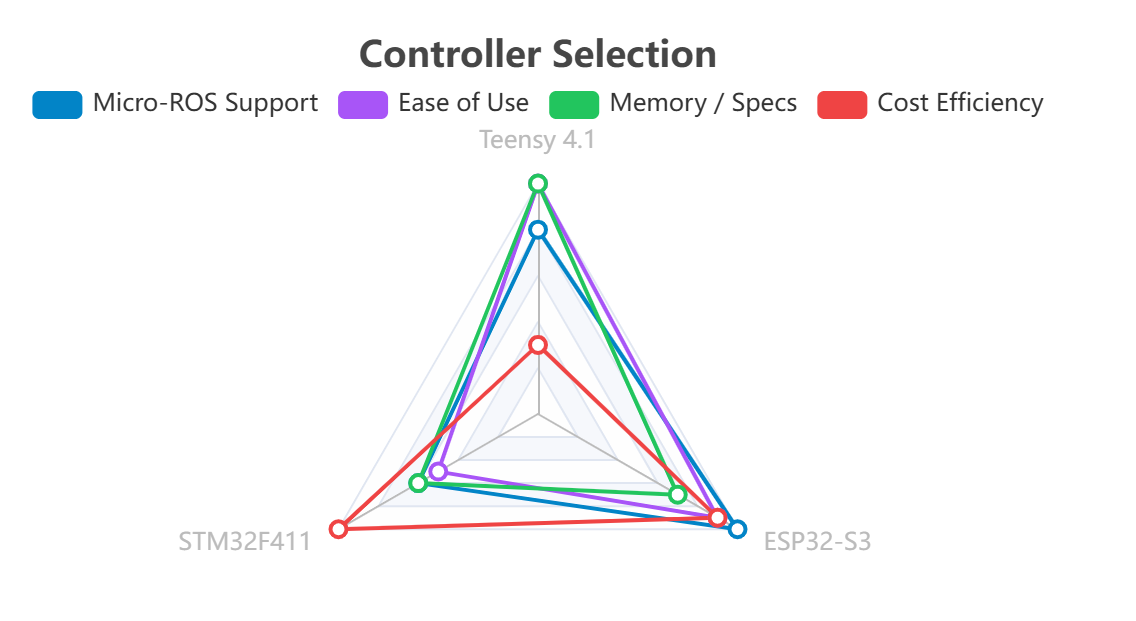
\includegraphics[width=0.7\linewidth]{figures/Chapter 4/Control_selection.png}
    \caption{Microcontroller Selection Comparison}
    \label{fig:control_selection}
\end{figure}

\newpage
\subsubsection{Summary of Microcontroller Selection}

\begin{figure}[H]
    \centering
    \begin{subfigure}[b]{0.3\textwidth}
        \centering
        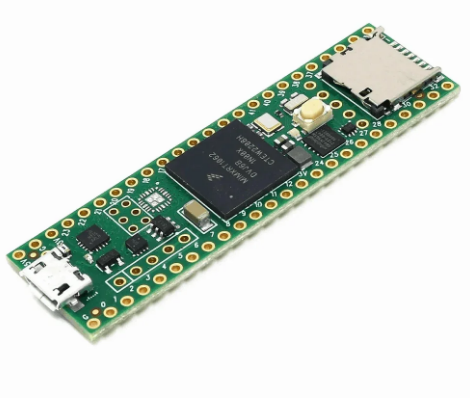
\includegraphics[width=\linewidth]{figures/Chapter 4/Teensy4_1.png}
        \caption{Teensy 4.1}
        \label{fig:teensy}
    \end{subfigure}
    \hfill
    \begin{subfigure}[b]{0.3\textwidth}
        \centering
        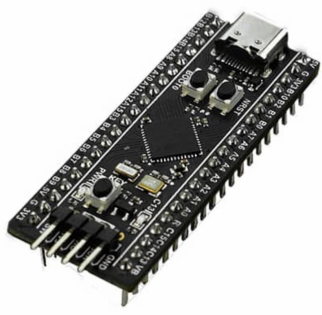
\includegraphics[width=\linewidth]{figures/Chapter 4/STM32F411.png}
        \caption{STM32F411}
        \label{fig:stm32}
    \end{subfigure}
    \hfill
    \begin{subfigure}[b]{0.3\textwidth}
        \centering
        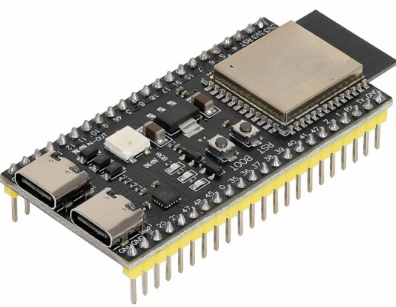
\includegraphics[width=\linewidth]{figures/Chapter 4/Esp32-s3.png}
        \caption{ESP32-S3 (Selected)}
        \label{fig:esp32}
    \end{subfigure}
    \caption{Microcontroller Candidates Evaluated}
    \label{fig:mcu_candidates}
\end{figure}

\paragraph{Teensy 4.1 (Score: 7.95/10)}
The Teensy 4.1 demonstrated superior raw computational performance, achieving a perfect score in technical specifications due to its 600 MHz Cortex-M7 processor. While this processing power offers significant headroom for complex kinematics, the platform's high unit cost (\textasciitilde\$30) resulted in a poor cost-efficiency rating. For a scalable swarm robotics architecture where per-unit cost is a critical constraint, the Teensy 4.1 presented a diminishing return on investment, as its surplus processing power exceeded the requirements of the low-level control loop.

\paragraph{STM32F411 (Score: 6.55/10)}
The STM32F411 ``Black Pill'' represents the industry-standard solution for embedded control, securing a perfect score for cost efficiency (\textasciitilde\$6). However, its integration into the AUSRA architecture was penalized by significant development overhead. The STM32 ecosystem (HAL/Cube IDE) requires a steeper learning curve compared to the Arduino framework, and the lack of native wireless connectivity necessitates an external bridge for micro-ROS communication. These factors would have introduced unacceptable latency into the development timeline without offering a distinct advantage in motor control precision.

\paragraph{ESP32-S3 (Selected --- Score: 8.80/10)}
The ESP32-S3 was identified as the optimal solution, balancing cost, performance, and connectivity \cite{espressif2023esp32}. Although its clock speed is lower than the Teensy, its \textbf{Dual-Core Xtensa LX7 architecture} provides a unique architectural advantage---it allows for the dedicated separation of tasks, with one core handling the blocking micro-ROS communication stack and the second core executing real-time motor control interrupts. Furthermore, its native support for Wi-Fi and USB-OTG simplified the hardware topology by eliminating the need for external communication bridges, justifying its selection as the primary low-level controller.

\newpage
\subsection{Motor Driver Selection}
\label{subsec:motor_driver}

The motor driver selection is critical for swarm robot efficiency, as the system operates on finite battery capacity and must maintain a compact form factor. The driver must offer high power efficiency and an optimal power-to-weight ratio.

\subsubsection{Candidates Evaluated}

Two motor driver families were evaluated:
\begin{itemize}
    \item \textbf{L298N:} A classic bipolar-transistor-based driver, widely available and popular for hobbyist applications.
    \item \textbf{Cytron MDD3A/MDD10A:} Modern MOSFET-based drivers offering superior efficiency and thermal performance.
\end{itemize}

\subsubsection{Selection Matrix}

\begin{table}[H]
\centering
\caption{Motor Driver Selection Matrix}
\label{tab:motor_driver_selection}
\resizebox{\textwidth}{!}{%
\begin{tabular}{|l|c|c|c|c|c|c|c|}
\hline
\multirow{2}{*}{\textbf{Criteria}} & \multirow{2}{*}{\textbf{Weight}} & \multicolumn{2}{c|}{\textbf{L298N}} & \multicolumn{2}{c|}{\textbf{Cytron MDD3A}} & \multicolumn{2}{c|}{\textbf{Cytron MDD10A}} \\ \cline{3-8} 
 & & Rating/5 & Score & Rating/5 & Score & Rating/5 & Score \\ \hline
Efficiency (Voltage drop) & 5 & 2 & 10 & 4 & 20 & 4 & 20 \\ \hline
Current Capacity & 4 & 3 & 12 & 4 & 16 & 5 & 20 \\ \hline
Price & 3 & 5 & 15 & 4 & 12 & 2 & 6 \\ \hline
Size \& Weight & 3 & 5 & 15 & 5 & 15 & 3 & 9 \\ \hline
\textbf{Final Scores} &  &  & \textbf{52} &  & \textbf{63} &  & \textbf{55} \\ \hline
\end{tabular}%
}
\end{table}

\subsubsection{Final Selection: Cytron MDD3A}

The \textbf{Cytron MDD3A} (Dual Channel 3A Motor Driver) was selected. The MDD10A's 10A rating was excessive for the selected actuators (stall current $<$2.5A), and each robot requires two drivers for three motors.

\begin{figure}[H]
    \centering
    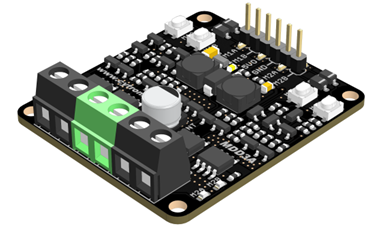
\includegraphics[width=0.4\linewidth]{figures/Chapter 4/MDD3A_Motor_Driver_2_Channel.png}
    \caption{Cytron MDD3A Dual Channel Motor Driver}
    \label{fig:mdd3a}
\end{figure}

\subsubsection{Justification of Selection}

\paragraph{Current Headroom}
The L298N (2.0A continuous) would operate at 90\% capacity with motors drawing 1.5--1.8A, risking overheating. The MDD3A (3.0A continuous, 5.0A peak) provides a 50\% safety margin.

\paragraph{Thermal Efficiency}
The L298N's BJT technology suffers from $\approx$2V voltage drop, wasting 17\% of power as heat on a 12V rail. The MDD3A's MOSFET technology ($R_{DS(on)} < 0.1\Omega$) delivers virtually all power to the motors, extending battery life and eliminating bulky heatsinks.

\paragraph{Protection Features}
The MDD3A includes active dynamic braking and fast-response protection circuits for precise stopping---essential for collision avoidance in swarm applications.

\paragraph{Size Optimization}
The MDD3A is 60\% smaller than the MDD10A, enabling a more compact chassis design and reduced weight.

\subsection{Power Source Selection}
\label{subsec:power_source}

\subsubsection{Design Constraint}
The primary power requirement was dictated by the NVIDIA Jetson Orin Nano, which operates most efficiently at higher input voltages ($>$12V) to minimize current draw and thermal dissipation. The local market availability in Egypt limited standard RC LiPo packs primarily to 3S (11.1V) configurations, which fall below the optimal efficiency threshold for the compute stack.

\subsubsection{Candidates Evaluated}

\begin{enumerate}
    \item \textbf{Single 3S LiPo (11.1V):} The standard hobbyist solution.
    \item \textbf{Dual 3S LiPo in Series (6S / 22.2V):} Connecting two packs to double the voltage.
    \item \textbf{Total P20S Industrial Pack (20V):} A commercial off-the-shelf power tool battery.
\end{enumerate}

\begin{figure}[H]
    \centering
    \begin{subfigure}[b]{0.45\textwidth}
        \centering
        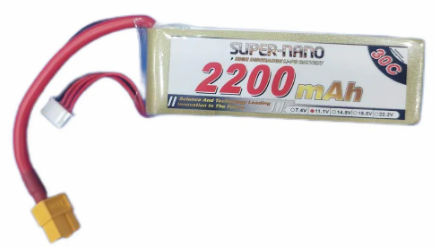
\includegraphics[width=\linewidth]{figures/Chapter 4/3S_Battery.png}
        \caption{Standard 3S LiPo Battery}
        \label{fig:3s_battery}
    \end{subfigure}
    \hfill
    \begin{subfigure}[b]{0.45\textwidth}
        \centering
        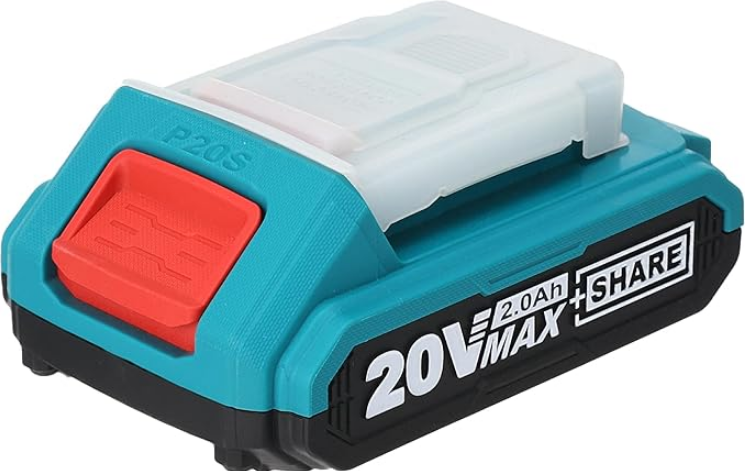
\includegraphics[width=\linewidth]{figures/Chapter 4/Total_p20s_battery.png}
        \caption{Total P20S Industrial Battery}
        \label{fig:p20s_battery}
    \end{subfigure}
    \caption{Power Source Candidates}
    \label{fig:battery_candidates}
\end{figure}

\subsubsection{Selection Matrix}

\begin{table}[H]
\centering
\caption{Power Source Comparison Matrix (Scale: 1 = Poor, 10 = Excellent)}
\label{tab:power_source_selection}
\begin{tabular}{|l|c|c|c|c|}
\hline
\textbf{Criteria} & \textbf{Weight} & \textbf{Single 3S LiPo} & \textbf{Dual 3S (Series)} & \textbf{Total P20S} \\ \hline
Voltage Sufficiency & 0.35 & 3 & 10 & 10 \\ \hline
Safety \& BMS & 0.25 & 6 & 2 & 10 \\ \hline
Charging Usability & 0.25 & 5 & 2 & 9 \\ \hline
Cost Efficiency & 0.15 & 8 & 4 & 9 \\ \hline
\textbf{Weighted Score} & \textbf{1.00} & \textbf{5.0} & \textbf{5.1} & \textbf{9.6} \\ \hline
\end{tabular}
\end{table}

\begin{figure}[H]
    \centering
    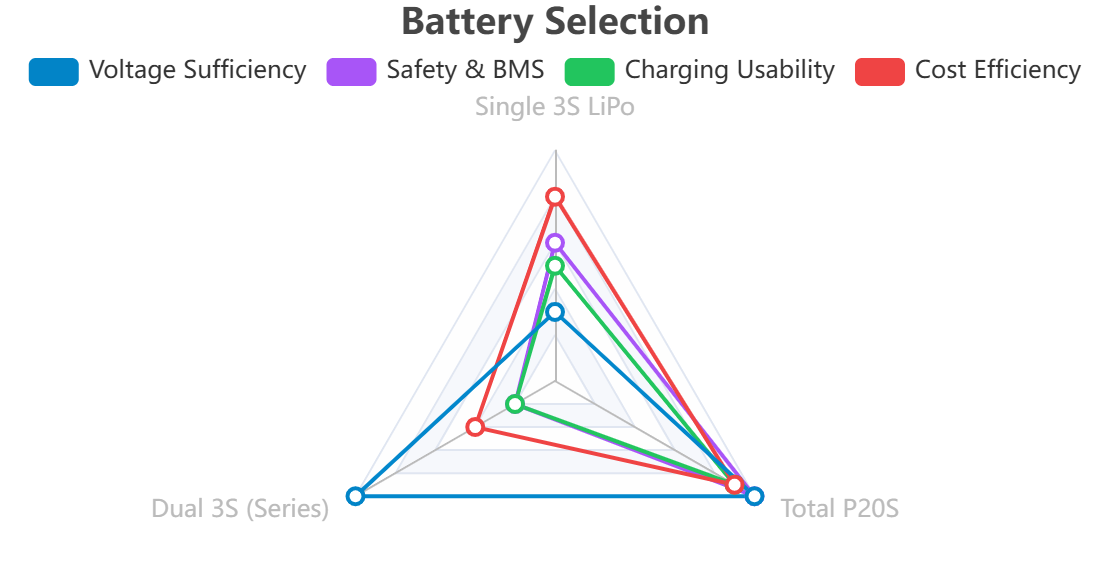
\includegraphics[width=0.7\linewidth]{figures/Chapter 4/Battery_selection.png}
    \caption{Battery Selection Comparison}
    \label{fig:battery_selection}
\end{figure}

\subsubsection{Justification of Selection}

\paragraph{Rejection of LiPo Configurations}
\begin{itemize}
    \item \textbf{Single 3S (11.1V):} Rejected as the nominal voltage (11.1V) forces the Jetson's internal regulators to draw higher current to maintain its power budget. This increases thermal stress and risks ``brownouts'' (voltage dips) when motors accelerate.
    \item \textbf{Dual Series (6S):} While a series configuration solves the voltage issue, it introduces significant safety and maintenance risks. Without a sophisticated industrial-grade BMS, two separate packs often discharge at uneven rates. This creates a scenario where one pack could drop below its critical voltage threshold while the other remains charged, leading to potential cell damage or fire hazards. Furthermore, the operational complexity of removing and balancing two separate packs for every charging cycle was deemed impractical for a user-friendly system.
\end{itemize}

\newpage
\paragraph{Selection of Total P20S (20V Platform)}
\begin{itemize}
    \item \textbf{Integrated BMS:} The battery features an internal Battery Management System that balances cells automatically, preventing the dangerous discharge scenarios inherent in custom series-LiPo setups.
    \item \textbf{Voltage Headroom:} The 20V nominal output ensures the Jetson and Motor Drivers operate in their high-efficiency capability region, significantly reducing amperage draw across the main bus.
    \item \textbf{``Charge-in-Place'' Architecture:} Unlike LiPos which require removal for safety, the P20S's ruggedized hard-shell casing and internal protections allowed us to design the ``Charging Mode'' circuit (referenced in Section \ref{subsec:isolation_logic}). This enables the robot to be charged safely via an external port without disassembling the chassis, mimicking commercial AMR (Autonomous Mobile Robot) standards.
\end{itemize}

\subsubsection{Battery Sizing (Target: $>$30 minutes runtime)}

\paragraph{Power Calculation}
The total power consumption was calculated by summing all major subsystems:

\begin{equation}
P_{total} = P_{Jetson} + P_{Motors} + P_{Camera} + P_{LiDAR} + P_{LowLevel}
\end{equation}

\begin{figure}[H]
    \centering
    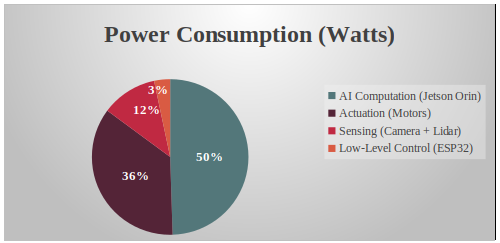
\includegraphics[width=0.6\linewidth]{figures/Chapter 4/Power_consumption.png}
    \caption{Power Consumption Breakdown}
    \label{fig:power_consumption}
\end{figure}

\textbf{Average Power:}
\begin{equation}
P_{avg} = 15 + 10.8 + 3 + 0.5 + 1 = 30.3 \approx 30 \text{ W}
\end{equation}

\textbf{Maximum Power:}
\begin{equation}
P_{max} = 25 + 72 + 5 + 1 + 1 = 104 \approx 105 \text{ W}
\end{equation}

\paragraph{Current Calculation}
Since the system is powered by a 20V source through Buck Converters, we calculate the current drawn from the battery, accounting for an estimated 90\% converter efficiency ($\eta = 0.9$).

\textbf{Average Current Draw:}
\begin{equation}
P_{batt,avg} = \frac{P_{avg}}{\eta} = \frac{30 \text{ W}}{0.9} = 33.3 \text{ W}
\end{equation}
\begin{equation}
I_{avg} = \frac{P_{batt,avg}}{V} = \frac{33.3 \text{ W}}{20 \text{ V}} = 1.67 \text{ A}
\end{equation}

\textbf{Peak Current Draw:}
\begin{equation}
P_{batt,max} = \frac{P_{max}}{\eta} = \frac{105 \text{ W}}{0.9} = 116.7 \text{ W}
\end{equation}
\begin{equation}
I_{max} = \frac{P_{batt,max}}{V} = \frac{116.7 \text{ W}}{20 \text{ V}} = 5.84 \text{ A}
\end{equation}

\paragraph{Capacity \& Runtime Verification}

\textbf{Selected Battery Specifications:}
\begin{itemize}
    \item \textbf{Model:} Total P20S (Lithium-Ion Power Tool Pack)
    \item \textbf{Voltage:} 20 V
    \item \textbf{Capacity:} 2000 mAh (2.0 Ah)
    \item \textbf{Discharge Rating:} High-Drain ($>$10C)
\end{itemize}

\textbf{Runtime Calculation:}
\begin{equation}
\text{Runtime} = \frac{\text{Capacity}}{I_{avg}} = \frac{2.0 \text{ Ah}}{1.67 \text{ A}} = 1.2 \text{ h} \approx 72 \text{ minutes}
\end{equation}

\textbf{Result:} The 2000mAh pack provides approximately 72 minutes of continuous operation, exceeding the 30-minute requirement by a factor of 2.4.

\paragraph{C-Rating (Discharge Safety) Check}
We must ensure the battery can handle the peak current (during acceleration/stall conditions) without damage.

\textbf{Required C-Rating:}
\begin{equation}
C_{req} = \frac{I_{max}}{\text{Capacity}} = \frac{5.84 \text{ A}}{2.0 \text{ Ah}} = 2.92 \text{ C}
\end{equation}

\textbf{Conclusion:} The required 2.92C is extremely low compared to the battery's rated capability ($>$10C), ensuring the pack will run cool and safe even during aggressive maneuvering.


\newpage
\section{Power Distribution and Safety Strategy}
\label{sec:power_distribution}

Effective power management is achieved through a combination of physical signal isolation and multi-stage voltage regulation.

\subsection{Physical Isolation Logic (Three-State Failsafe)}
\label{subsec:isolation_logic}

Safety is enforced via a \textbf{6-pin E-TEN1322 Toggle Switch (ON-OFF-ON)}. This component acts as a hardware multiplexer, defining three mutually exclusive operational states to prevent user error and electrical hazards.

\begin{figure}[H]
    \centering
    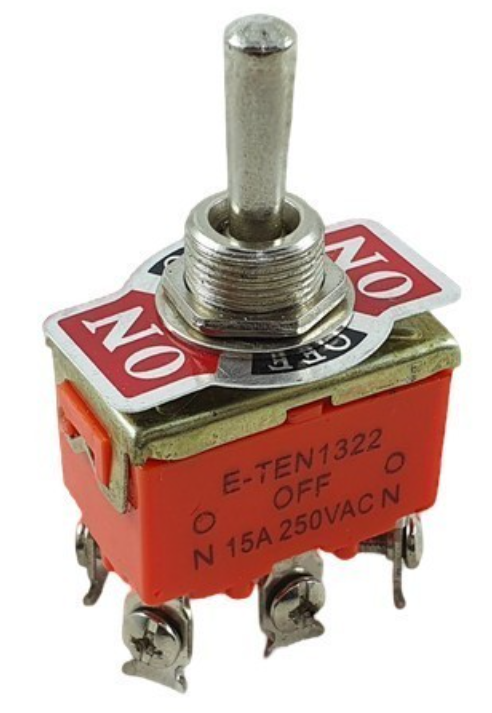
\includegraphics[width=0.3\linewidth]{figures/Chapter 4/Power_switch.png}
    \caption{Three-State Power Switch Configuration}
    \label{fig:power_switch}
\end{figure}

\begin{itemize}
    \item \textbf{State 1: Charge Mode} --- The battery terminals are electrically disconnected from the robot's internal power bus and routed exclusively to the external GX16 Aviation Port. This ensures 100\% isolation of the sensitive computing units (Jetson/ESP32) from potential voltage spikes or ground loops during the charging cycle.
    
    \item \textbf{State 2: Idle} --- In the neutral position, the battery is fully disconnected from both the charging port and the internal system. This serves as a \textbf{Master Kill Switch}, preventing accidental startup during transport, maintenance, or code flashing. It also mitigates parasitic battery drain when the robot is in storage.
    
    \item \textbf{State 3: Run Mode} --- The charging port is physically disconnected, and the battery power is routed to the internal 20V DC Bus. This activates the dual-stage regulation system to power the robot's logic and actuation subsystems.
\end{itemize}

\subsection{Dual-Stage Voltage Regulation}
\label{subsec:voltage_regulation}

To maintain system stability and component safety, the 20V bus is conditioned by two independent regulation stages:

\begin{figure}[H]
    \centering
    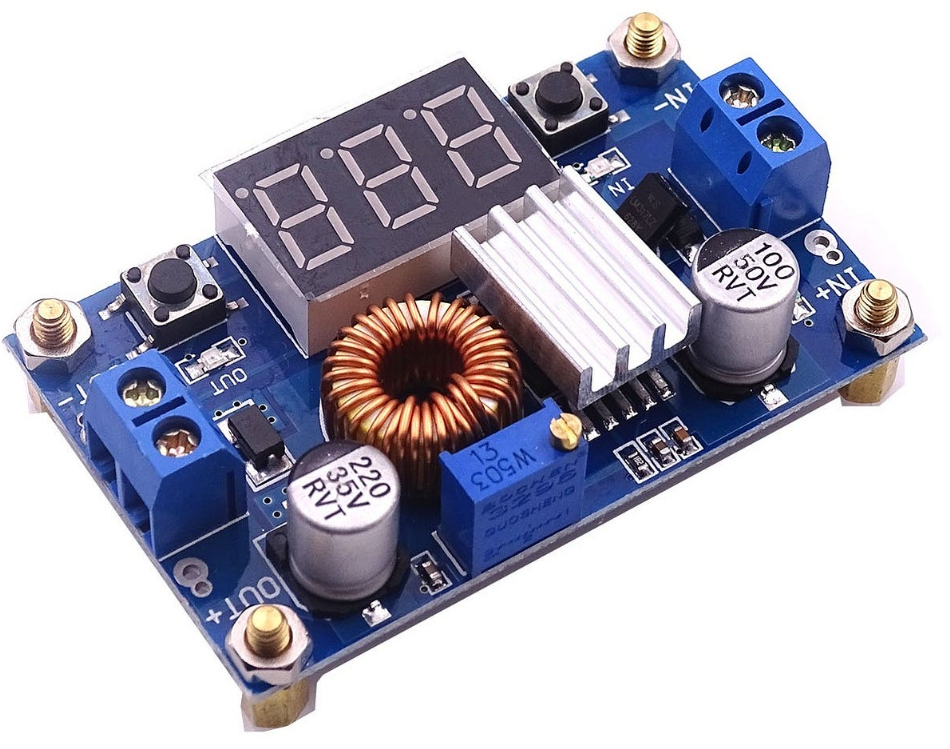
\includegraphics[width=0.7\linewidth]{figures/Chapter 4/Buck_convertor.png}
    \caption{Buck Converter Modules for Voltage Regulation}
    \label{fig:buck_converter}
\end{figure}

\begin{itemize}
    \item \textbf{Logic Regulator:} A precision step-down converter provides a stable supply for the NVIDIA Jetson Orin Nano. This isolation protects the compute stack from voltage ``brownouts'' that occur on the main line when motors draw high inrush currents during acceleration.
    
    \item \textbf{Actuation Regulator:} A dedicated high-power buck converter steps the 20V battery voltage down to a regulated 12V supply, matching the nominal voltage rating of the DC motors. This regulation guarantees that the motors receive a consistent voltage regardless of the battery's fluctuating charge level (21V to 18V), ensuring predictable kinematic performance throughout the entire discharge cycle.
\end{itemize}


\newpage
\section{Low-Level Firmware Design}
\label{sec:lowlevel_design}

This section presents the theoretical foundation and implementation strategy for the low-level motor control firmware running on the ESP32-S3 microcontroller.

\subsection{Actuator Feedback: Quadrature Encoders}
\label{subsec:encoders}

Encoders are sensors mounted on a motor's rear shaft to sense rotation. As the shaft moves, the encoder generates a pulse train signal that provides position and velocity feedback for closed-loop control.

\begin{figure}[H]
    \centering
    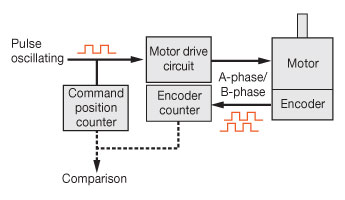
\includegraphics[width=0.6\linewidth]{figures/Chapter 4/Motor_encoder_topology.jpg}
    \caption{Motor Encoder Topology}
    \label{fig:encoder_topology}
\end{figure}

\subsubsection{Operating Principle}

The number of pulses indicates the motor shaft position and rotation distance from a home position. For example, with an encoder resolution of 935 PPR (Pulses Per Revolution), 935 pulses indicate one complete revolution. The pulse frequency (Hz) indicates rotational speed, while the phase relationship between channels A and B determines direction.

\paragraph{Optical Encoder Technology}
The AUSRA platform uses optical encoders, which provide the highest precision and resolution. In a transmissive optical encoder, the main components are:
\begin{itemize}
    \item A light emitter (LED)
    \item A code wheel with precision slits
    \item A light receiver (photo sensor)
\end{itemize}

As the code wheel rotates, light either passes through the slits or is blocked, creating a binary pulse train that the microcontroller interprets as position data.

\begin{figure}[H]
    \centering
    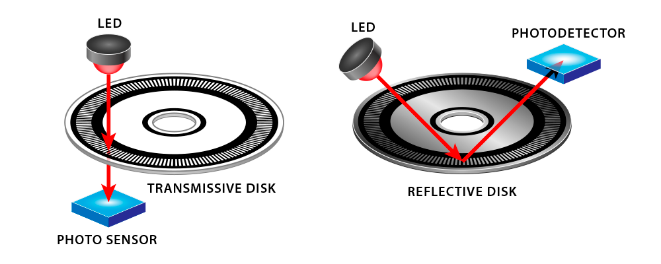
\includegraphics[width=0.7\linewidth]{figures/Chapter 4/Transimisive_vs_reflective.png}
    \caption{Transmissive vs. Reflective Encoder Configurations}
    \label{fig:encoder_types}
\end{figure}

\subsection{Encoder Data Acquisition Strategy}
\label{subsec:encoder_acquisition}

With 935 PPR encoders and target speeds up to 300 RPM, the signal frequency reaches approximately 4,675 Hz---a new pulse every 213 microseconds. Two architectural approaches were evaluated:

\subsubsection{Polling vs. Interrupt-Driven Architecture}

\paragraph{Polling (Rejected)}
In polling, the CPU continuously checks GPIO pin states in the main loop. However, the ESP32 handles Wi-Fi, micro-ROS communication, and PID calculations. If any task blocks the CPU for more than 200$\mu$s, pulses are missed, causing incorrect velocity readings and erratic behavior.

\paragraph{Interrupt Service Routines (Selected)}
We adopted an event-driven architecture using hardware interrupts. When a pin voltage transitions, the GPIO controller triggers the CPU to immediately execute an Interrupt Service Routine (ISR), increment the counter, and return to the main task. This guarantees atomic data capture with nanosecond-scale latency regardless of CPU load.

\paragraph{Critical Implementation: IRAM\_ATTR}
ESP32 program code typically resides in external Flash memory. If an interrupt fires while Flash is busy, the system crashes. The solution is the \texttt{IRAM\_ATTR} macro:

\begin{lstlisting}[language=C, caption={ISR with IRAM\_ATTR for Flash-Independent Execution}]
void IRAM_ATTR motor0_isr() {
    encoder_count[0]++;
}
\end{lstlisting}

This directive places the ISR code in internal SRAM, ensuring zero-latency access even during Flash operations.

\subsection{Quadrature Encoding Selection}
\label{subsec:quadrature_selection}

Quadrature encoders produce two channels (A and B) offset by 90°, enabling direction sensing. Three encoding types exist: X1, X2, and X4, differing in which edges are counted.

\subsubsection{X1 Encoding Selection Rationale}

We selected X1 encoding (counting only rising edges of Channel A) over X4 for three reasons:

\paragraph{1. Computational Efficiency}
At 300 RPM with three motors:
\begin{itemize}
    \item \textbf{X4 Mode:} $3740 \times 5 \times 3 = 56,100$ ISR calls/second
    \item \textbf{X1 Mode:} $935 \times 5 \times 3 = 14,025$ ISR calls/second
\end{itemize}

X1 reduces CPU overhead by 75\%, preserving cycles for Wi-Fi and micro-ROS communication.

\paragraph{2. Noise Immunity}
X4 is vulnerable to the ``dither problem''---when a motor stops on an encoder edge, vibration causes rapid signal toggling, accumulating phantom counts. X1 requires a full signal cycle to register a count, acting as a natural hysteresis filter.

\paragraph{3. Sufficient Resolution}
At 935 ticks/rev ($\approx 0.38°$/tick), even at low speeds (60 RPM) with a 50Hz control loop, the encoder registers $\approx$18 ticks per cycle---sufficient granularity for smooth PID control.

\subsection{Encoder Calibration}
\label{subsec:encoder_calibration}

Accurate PPR determination is critical for odometry. We used the ``Encoder Shaft'' method---tracking rotation directly at the encoder disc, bypassing gearbox backlash errors.

\paragraph{Procedure:}
\begin{enumerate}
    \item Remove the motor's rear cap to expose the encoder disc
    \item Attach a micro-marker to the rotating magnet
    \item Rotate exactly one revolution (360°) while recording tick count
    \item Repeat 20 times per motor and average results
\end{enumerate}

\paragraph{Result:} The calibration converged to \textbf{935 PPR}, which was hardcoded into the firmware.

\subsection{Velocity Estimation and Signal Processing}
\label{subsec:velocity_estimation}

Deriving velocity $\omega = \frac{d\theta}{dt}$ from discrete encoder ticks introduces quantization noise, particularly problematic for the PID derivative term.

\subsubsection{The Quantization Problem}

At 60 RPM with a 50Hz control loop, readings fluctuate between 18-19 ticks per cycle. This ``staircase'' signal creates high-frequency spikes in the derivative calculation, causing motor humming and instability.

\subsubsection{Solution: First-Order Low-Pass Filter}

We implemented an Exponential Moving Average (EMA) filter:

\begin{equation}
\hat{\omega}[k] = \alpha \cdot \omega_{raw}[k] + (1-\alpha) \cdot \hat{\omega}[k-1]
\label{eq:lowpass_filter}
\end{equation}

Where:
\begin{itemize}
    \item $\hat{\omega}[k]$ = filtered velocity estimate
    \item $\omega_{raw}[k]$ = raw velocity from encoder ticks
    \item $\alpha$ = smoothing factor (0 to 1)
\end{itemize}

\paragraph{Tuning:} Through step response analysis, we selected $\alpha = 0.1$. This provides sufficient noise rejection to stabilize the derivative term while introducing only $\approx$60ms phase lag---well within the stability margins of the robot's mechanical inertia.


\newpage
\section{Control Strategy and Controller Selection}
\label{sec:control_strategy}

To regulate the angular velocity of the omnidirectional wheels, a comparative analysis of three standard control architectures was conducted: Proportional-Integral-Derivative (PID), Linear Quadratic Regulator (LQR), and Model Predictive Control (MPC). The selection criteria focused on computational efficiency, model dependency, and suitability for the ESP32-S3 hardware constraints.

\subsection{Controller Selection Analysis}
\label{subsec:controller_selection}

Table~\ref{tab:controller_selection} presents a weighted decision matrix comparing the three controller architectures across four critical criteria.

\begin{table}[H]
    \centering
    \caption{Controller Selection Matrix}
    \label{tab:controller_selection}
    \begin{tabular}{|l|c|c|c|c|}
        \hline
        \textbf{Selection Criteria} & \textbf{Weight} & \textbf{MPC} & \textbf{LQR} & \textbf{PID} \\
        \hline
        Computational Cost & 30\% & 1 & 3 & 5 \\
        \hline
        Model Dependency & 30\% & 1 & 2 & 5 \\
        \hline
        Constraint Handling & 15\% & 4 & 2 & 2 \\
        \hline
        Application Suitability & 25\% & 1 & 2 & 5 \\
        \hline
        \textbf{Final Score} & --- & \textbf{1.45} & \textbf{2.30} & \textbf{4.55} \\
        \hline
    \end{tabular}
\end{table}

\subsubsection{Computational Cost}
\begin{itemize}
    \item \textbf{PID:} Extremely low. Requires only basic arithmetic (multiplication/addition) for three terms. Easily runs at $>$1kHz on ESP32.
    \item \textbf{LQR:} Low/Medium. Requires matrix multiplication of the state vector by the gain matrix $\mathbf{K}$. Efficient but requires full state feedback.
    \item \textbf{MPC:} Very high. Requires solving a Quadratic Programming (QP) optimization problem at every time step. Infeasible to run three parallel instances at 50Hz on an ESP32 while managing the Wi-Fi stack.
\end{itemize}

\subsubsection{Model Dependency}
\begin{itemize}
    \item \textbf{PID:} Model-free. Does not require a physics model of the motor (inductance, inertia, friction). Tunable via heuristics.
    \item \textbf{LQR:} High dependency. Requires an accurate state-space representation. If the physical motor parameters (friction coefficient, moment of inertia) change or are unknown, performance degrades significantly.
    \item \textbf{MPC:} Critical dependency. Relies entirely on the predictive model. Any mismatch between the model and reality leads to poor prediction and instability.
\end{itemize}

\subsubsection{Constraint Handling}
\begin{itemize}
    \item \textbf{PID:} Saturation (clamping) is added manually to handle voltage limits (Anti-Windup).
    \item \textbf{LQR:} None. Does not inherently handle actuator saturation.
    \item \textbf{MPC:} Native constraint handling capability, but this feature is unnecessary for simple speed regulation where clamping suffices.
\end{itemize}

\subsubsection{Application Suitability}
\begin{itemize}
    \item \textbf{PID:} Ideal for SISO (Single-Input Single-Output) systems where the objective is setpoint tracking (maintaining RPM).
    \item \textbf{LQR:} Best suited for MIMO (Multi-Input Multi-Output) regulation and stabilization (e.g., balancing an inverted pendulum) rather than simple reference tracking.
    \item \textbf{MPC:} Best suited for complex trajectory planning where future states must be optimized (e.g., autonomous driving pathing), not low-level actuator control.
\end{itemize}

\subsubsection{Selection Conclusion}
The \textbf{PID Controller} was selected because the motor system is treated as three independent SISO systems. The prohibitive computational cost of MPC and the high model-dependency of LQR were unjustified for a system where the physical parameters (friction, load) fluctuate dynamically during operation.

\subsection{Mathematical Derivation: Discrete PID Algorithm}
\label{subsec:discrete_pid}

The standard continuous-time PID equation is defined as:
\begin{equation}
    u(t) = K_p \cdot e(t) + K_i \int e(t) \, dt + K_d \cdot \frac{de(t)}{dt}
    \label{eq:pid_continuous}
\end{equation}

However, microcontrollers operate in discrete time steps. To implement this on the ESP32-S3, the equation was discretized using the Backward Euler Method with a sampling time $T_s = 20$ms (50Hz).

\subsubsection{Proportional Term}
\begin{equation}
    P[k] = K_p \cdot e[k]
    \label{eq:pid_p}
\end{equation}

\subsubsection{Integral Term (Accumulation)}
The integral is approximated as the sum of errors multiplied by the sampling time:
\begin{equation}
    I[k] = I[k-1] + K_i \cdot e[k] \cdot T_s
    \label{eq:pid_i}
\end{equation}

This recursive addition allows the controller to eliminate steady-state error ($e_{ss}$) by accumulating output until the error reaches zero.

\subsubsection{Derivative Term (Difference)}
The derivative is approximated as the slope between the current and previous error:
\begin{equation}
    D[k] = K_d \cdot \frac{e[k] - e[k-1]}{T_s}
    \label{eq:pid_d}
\end{equation}

\subsubsection{Final Control Law}
The total control signal (PWM Duty Cycle) sent to the motor driver is:
\begin{equation}
    u[k] = P[k] + I[k] + D[k]
    \label{eq:pid_control_law}
\end{equation}

\subsection{Stability Augmentation: Anti-Windup Strategy}
\label{subsec:anti_windup}

A critical limitation of the standard Integral term is \textit{windup}. When the actuator reaches its physical limit (e.g., Max PWM = 255) but the error persists (e.g., the robot is blocked by an obstacle), the Integral term continues to accumulate virtually to infinity. When the obstacle is removed, the controller remains saturated for a prolonged period, causing dangerous overshooting.

To mitigate this, a \textbf{Clamping Anti-Windup} mechanism was implemented:
\begin{enumerate}
    \item \textbf{Calculate Tentative Output:} Compute $u_{calc} = P + I + D$
    \item \textbf{Check Saturation:} If $|u_{calc}| > u_{max}$:
    \begin{itemize}
        \item Clamp the final output $u[k]$ to $u_{max}$
        \item Freeze the Integral: Stop adding to $I[k]$ to prevent it from growing beyond the physical capacity of the system
    \end{itemize}
\end{enumerate}

The specific C++ implementation of the clamping logic is provided in Appendix A (Motor.cpp).

\subsection{Tuning Methodology}
\label{subsec:pid_tuning}

A significant engineering challenge was the \textbf{Concurrent Development Phase}, where the low-level firmware was being developed simultaneously with the mechanical assembly. This prevented traditional model-based tuning because the mass and inertia of the robot were constantly changing. A hybrid tuning approach was adopted.

\subsubsection{Phase 1: Heuristic Tuning (Ziegler-Nichols Variant)}
Performed on a test bench with ``free spinning'' wheels:
\begin{enumerate}
    \item Set $K_i$ and $K_d$ to zero
    \item Increase $K_p$ until the motor velocity oscillates around the setpoint
    \item Set $K_p$ to $0.5 \times K_{oscillation}$ to ensure stability
    \item Introduce $K_i$ incrementally to remove steady-state error (the difference between Target RPM and Actual RPM)
\end{enumerate}

\subsubsection{Phase 2: Pole Placement using MATLAB PID Tuner}
Once the robot was fully assembled (loaded condition), the MATLAB System Identification Toolbox was utilized:
\begin{enumerate}
    \item \textbf{Step Response Test:} A step input (0 to 100 PWM) was injected and the open-loop velocity response curve was logged.
    \item \textbf{Transfer Function Estimation:} The motor-wheel system was approximated as a first-order plant with dead time:
    \begin{equation}
        G(s) = \frac{K}{\tau s + 1}
        \label{eq:transfer_function}
    \end{equation}
    \item \textbf{Optimization:} The MATLAB PID Tuner app was used to solve for optimal gains that provided a Rise Time $< 0.2$s and Overshoot $< 5\%$.
\end{enumerate}
\newpage
\section{The Micro-ROS Architecture}
\label{sec:microros}

This section explains the communication bridge between the MCU and the high-level computer (Jetson/Laptop).

\subsection{Overview: Bridging Real-Time Embedded Systems with DDS}
\label{subsec:microros_overview}

The integration of resource-constrained microcontrollers (MCUs) into the Robot Operating System (ROS 2) ecosystem presents a fundamental architectural challenge. Standard ROS 2 nodes communicate using the Data Distribution Service (DDS) protocol---specifically RTPS (Real-Time Publish-Subscribe). DDS is a heavy, peer-to-peer protocol requiring significant memory for discovery caches, serialization buffers, and history scaling, often exceeding 1MB of RAM---far beyond the capacity of typical MCUs.

To resolve this, \textbf{micro-ROS} was implemented, a specialized variant designed to extend the DDS ``Global Data Space'' onto the ESP32-S3. Unlike simple serial bridges (e.g., rosserial) which use custom, non-standard framing, micro-ROS creates first-class ROS 2 nodes on the microcontroller, allowing them to interact seamlessly with the high-level system using standard message definitions.

\subsection{The Client-Agent Architecture}
\label{subsec:client_agent}

The micro-ROS framework abandons the peer-to-peer model of standard DDS in favor of a \textbf{Client-Agent topology}. This asymmetrical architecture offloads the heavy lifting of discovery and routing to a more powerful host machine.

\subsubsection{The Micro-ROS Client (ESP32-S3)}
\begin{itemize}
    \item Runs a lightweight implementation of the ROS 2 stack (based on \texttt{rclc})
    \item Does not store the ROS graph or discovery database
    \item Serializes messages and sends them point-to-point to the Agent
\end{itemize}

\subsubsection{The Micro-ROS Agent (Jetson/Laptop)}
The Agent acts as a \textbf{Stateful Proxy} or ``Broker,'' running as a standard ROS 2 node on the host computer with the following responsibilities:
\begin{enumerate}
    \item \textbf{Translation:} Converts the lightweight Micro-XRCE-DDS messages from the MCU into standard DDS RTPS packets for the rest of the ROS 2 network
    \item \textbf{Discovery:} Handles the ROS 2 discovery traffic (Participant announcements) on behalf of the MCU
    \item \textbf{Entity Management:} Maintains the state of Publishers, Subscribers, and Services created by the MCU
\end{enumerate}

\begin{figure}[H]
    \centering
    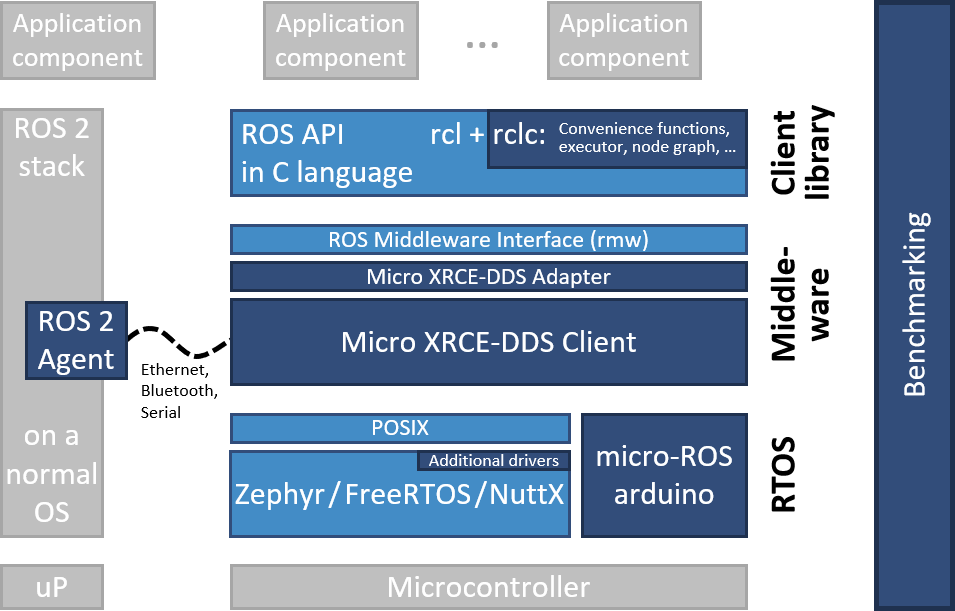
\includegraphics[width=0.85\linewidth]{figures/Chapter 4/Micro_ros_architecture.png}
    \caption{Micro-ROS Client-Agent Architecture}
    \label{fig:microros_architecture}
\end{figure}

\subsection{The Middleware: Micro-XRCE-DDS}
\label{subsec:xrce_dds}

At the heart of the communication layer lies \textbf{Micro-XRCE-DDS} (eXtremely Resource Constrained Environments---Data Distribution Service), an ISO standard protocol (OMG DDS-XRCE) optimized for embedded devices.

\subsubsection{Protocol Efficiency}
Unlike standard DDS, which creates dynamic connections for every topic, XRCE-DDS utilizes a stateless connection model for data transmission to minimize overhead:
\begin{itemize}
    \item \textbf{Serialization:} Uses CDR (Common Data Representation) with reduced header sizes compared to RTPS
    \item \textbf{Memory Footprint:} Designed to operate with $<$50KB of RAM, making it feasible to run alongside the Wi-Fi stack and motor control tasks on the ESP32-S3
\end{itemize}

\subsubsection{Transport Layer Agnosticism}
A critical engineering feature of Micro-XRCE-DDS is its separation from the physical transport layer. This allowed the construction of a dual-transport system:

\paragraph{UDP over Wi-Fi (UDPv4)}
\begin{itemize}
    \item \textbf{Selected for:} Development and Telemetry
    \item \textbf{Mechanism:} Uses IP addressing to stream data wirelessly, enabling ``Hardware-in-the-Loop'' style debugging where the robot moves freely while streaming live encoder data to the laptop
\end{itemize}

\paragraph{UART Serial}
\begin{itemize}
    \item \textbf{Selected for:} Deployment
    \item \textbf{Mechanism:} Uses a direct wired connection (Tx/Rx) to the Jetson, eliminating latency jitter and radio interference risks in industrial environments
    \item \textbf{Note:} The application logic remains identical; only the transport configuration struct is modified
\end{itemize}

\subsection{Deep Dive: The Micro-ROS Agent}
\label{subsec:agent_deep_dive}

The Agent is not merely a pass-through pipe; it is a complex server that manages the lifecycle of the embedded node.

\subsubsection{Connection Mechanics and Handshake}
Connecting to the Agent is a rigorous, multi-step handshake process handled by the \texttt{rmw\_microxrcedds} layer:

\paragraph{Session Initiation}
\begin{enumerate}
    \item The ESP32 sends a \texttt{CREATE\_SESSION} request containing a unique Session ID and Client Key
    \item The Agent checks if a session with that ID already exists; if not, it allocates memory structures to track the new client
    \item \textbf{Implementation Detail:} A static Agent IP (192.168.x.x) was hardcoded for Wi-Fi trials to bypass the complexity of UDP broadcast discovery, ensuring faster boot times ($<$2 seconds)
\end{enumerate}

\paragraph{Entity Creation (The ``Graph'' Build)}
Once the session is established, the MCU sends discrete requests to create entities:
\begin{itemize}
    \item \texttt{create\_participant}
    \item \texttt{create\_topic} (e.g., \texttt{/cmd\_vel})
    \item \texttt{create\_publisher} / \texttt{create\_subscriber}
\end{itemize}

The Agent executes these requests on the ROS 2 network. If the Agent crashes, these entities disappear from the ROS graph immediately, providing an inherent ``Liveliness'' check.

\subsubsection{Running the Agent}
For the implementation, a Dockerized version of the Agent was utilized to ensure environment consistency across different development machines (Ubuntu 22.04 / Linux Mint):
\begin{lstlisting}[language=bash, caption={Micro-ROS Agent Launch Command}]
ros2 run micro_ros_agent micro_ros_agent udp4 --port 8888
\end{lstlisting}

Port 8888 is the standard UDP listening port that the ESP32 targets in its transport configuration.

\subsection{Implementation Strategy: The rclc Executor}
\label{subsec:rclc_executor}

On the ESP32 side, the \texttt{rclc} (ROS Client Library for C) was utilized, which provides a C-API wrapper around the middleware. This is distinct from the C++ (\texttt{rclcpp}) or Python (\texttt{rclpy}) libraries used on the PC.

\subsubsection{Memory Management (Allocators)}
Dynamic memory allocation (\texttt{malloc}) is dangerous in embedded systems due to heap fragmentation. Micro-ROS requires a custom allocator---the FreeRTOS-compatible allocator was configured to reserve a static memory block for the ROS stack, ensuring that message generation never causes a ``Heap Overflow'' during runtime.

\subsubsection{The Executor Pattern}
Unlike the callback-based spin of standard ROS 2, \texttt{rclc} gives the developer granular control over execution:

\begin{lstlisting}[language=C, caption={rclc Executor Initialization (Simplified)}]
// Initialize executor with 2 handles
rclc_executor_init(&executor, &context, 2, &allocator);

// Add subscription and timer
rclc_executor_add_subscription(&executor, &sub_cmd_vel, &msg, &callback);
rclc_executor_add_timer(&executor, &timer_pub);
\end{lstlisting}

\paragraph{Determinism:} The Executor was configured to run in the main \texttt{loop()} with a short timeout. This polling-based execution (\texttt{rclc\_executor\_spin\_some}) allows deterministic interleaving of communication tasks with motor control tasks, preventing the Wi-Fi stack from starving the PID loop.

\subsection{Quality of Service (QoS) and Reliability}
\label{subsec:qos}

One of the most significant technical decisions in this architecture was the tuning of the Quality of Service (QoS) policies for Wi-Fi transport.

\subsubsection{The Problem: ``Reliable'' Overhead}
By default, ROS 2 uses a \textbf{Reliable} policy where the middleware guarantees delivery. If a packet is dropped (common in Wi-Fi), the sender halts and retries.

\textbf{Consequence:} On a mobile robot, a momentary Wi-Fi glitch would cause the \texttt{cmd\_vel} stream to pause. When the connection resumes, the robot might receive a burst of old, outdated velocity commands, causing dangerous, jerky behavior.

\subsubsection{The Solution: ``Best Effort'' (UDP-Style)}
The micro-ROS publishers and subscribers were explicitly configured to use \texttt{rmw\_qos\_profile\_sensor\_data} (Best Effort):
\begin{itemize}
    \item \textbf{Behavior:} The system attempts to send the packet once; if lost, it is discarded
    \item \textbf{Rationale:} For real-time velocity commands, if a packet arrives late, it is useless. It is better to skip a frame and wait for the fresh command than to delay the entire system trying to recover old data
\end{itemize}

This configuration proved vital for the smoothness of the ``Square Path'' demonstration.

\subsection{Section Summary}
\label{subsec:microros_summary}

This architecture effectively creates a distributed computing system where the ``Brain'' (Jetson) and ``Muscle'' (ESP32) are loosely coupled by a standardized protocol (DDS-XRCE), yet tightly integrated in terms of data flow. The use of the Agent as an intermediary allows the heavy ROS 2 stack to remain on the host, while the Client remains lightweight enough to run alongside critical 50Hz motor control loops.

\begin{figure}[H]
    \centering
    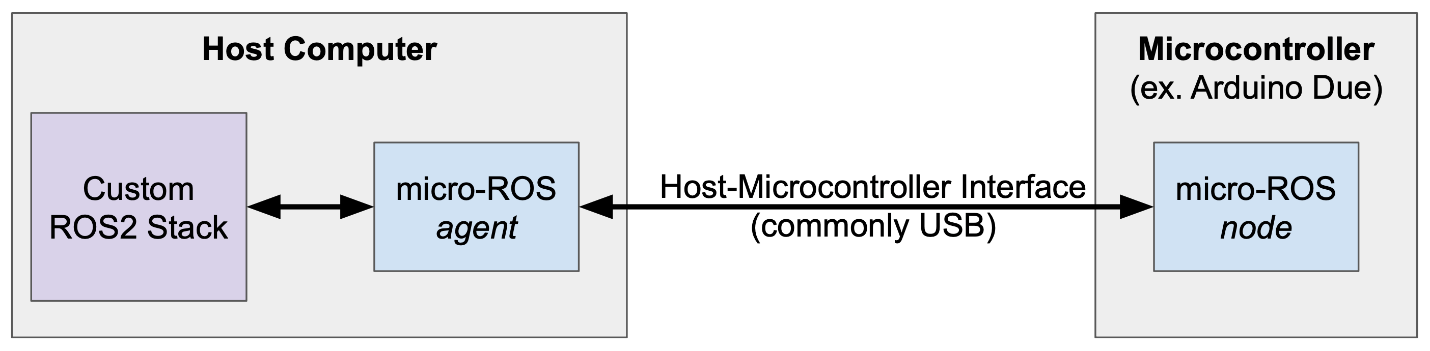
\includegraphics[width=0.7\linewidth]{figures/Chapter 4/Section_summary.png}
    \caption{Micro-ROS Communication Summary}
    \label{fig:microros_summary}
\end{figure}

\newpage
\section{Evolutionary Architecture: The Three-Phase Iteration}
\label{sec:evolutionary_architecture}

The development of the low-level control subsystem followed an iterative process of architectural exploration, driven by competing constraints of hard real-time performance, soft real-time communication, and development velocity.

\subsection{Trial 1: RTOS-Native Approach}
\label{subsec:trial1}

\subsubsection{Hypothesis}
Running micro-ROS as a prioritized task directly within the FreeRTOS kernel would offer the highest determinism by eliminating Arduino framework overhead.

\subsubsection{Implementation}
The \texttt{micro\_ros\_setup} component was integrated into ESP-IDF with a preemptive scheduling architecture:
\begin{itemize}
    \item \texttt{Task\_Transport} (Priority 2): Wi-Fi and UDP handling
    \item \texttt{Task\_MicroROS} (Priority 3): rclc executor processing
    \item \texttt{Task\_MotorControl} (Priority 5): Hard real-time PID at 50Hz
\end{itemize}

\subsubsection{Failure Mode}
\begin{itemize}
    \item \textbf{Stack Overflows:} The XRCE-DDS serialization layer is stack-intensive; tuning stack depth was precarious
    \item \textbf{Build Complexity:} Cross-compiling for the specific FreeRTOS kernel required complex CMake modifications with $>$3 minute build times
    \item \textbf{Conclusion:} Maintenance overhead outweighed marginal scheduling gains
\end{itemize}

\subsection{Trial 2: Bare-Metal ESP-IDF Optimization}
\label{subsec:trial2}

\subsubsection{Hypothesis}
Using ESP-IDF's native hardware peripherals without ROS abstraction would maximize hardware efficiency with near-zero CPU load.

\subsubsection{Implementation}
\begin{itemize}
    \item \textbf{PCNT Peripheral:} Hardware pulse counter for encoder reading with zero CPU overhead
    \item \textbf{LEDC Peripheral:} Hardware PWM generation with jitter-free duty cycles
\end{itemize}

\subsubsection{Failure Mode}
\begin{itemize}
    \item \textbf{Software Gap:} ESP-IDF's C-based framework required writing PID, kinematics, and vector math libraries from scratch
    \item \textbf{Brittleness:} Custom low-level drivers made pin configuration changes require register-level rewrites
    \item \textbf{Conclusion:} The ESP32-S3's dual-core 240MHz processor was powerful enough without extreme PCNT optimization; development time cost was unjustified
\end{itemize}

\subsection{Trial 3: Hybrid Architecture (Final Solution)}
\label{subsec:trial3}

The final architecture leverages Arduino Core for rapid hardware abstraction while retaining micro-ROS for robust communication.

\subsubsection{Dual-Core Asymmetric Processing}
\begin{itemize}
    \item \textbf{Core 0 (Protocol):} Wi-Fi stack and micro-ROS Agent communication
    \item \textbf{Core 1 (Application):} PID calculations and Encoder ISRs
\end{itemize}

This isolation ensures Wi-Fi packet bursts never interrupt encoder tick reading.

\subsubsection{IRAM-Resident ISRs}
The \texttt{IRAM\_ATTR} macro places ISRs in high-speed internal SRAM, eliminating cache-miss crashes and reducing interrupt latency to nanoseconds.

\subsubsection{Atomic Data Access}
Race conditions are prevented using critical sections:
\begin{lstlisting}[language=C, caption={Atomic Encoder Read}]
noInterrupts();  // Critical section start
long safe_counts = encoder_count;
interrupts();    // Critical section end
\end{lstlisting}

\subsubsection{Validation Results}
\begin{itemize}
    \item \textbf{Stability:} $>$30 minutes continuous operation without crashes
    \item \textbf{Responsiveness:} End-to-end latency $<$15ms (keypress to motor)
    \item \textbf{Safety:} 500ms software watchdog integration for failsafe operation
\end{itemize}

\section{Summary}
\label{sec:electrical_summary}

This chapter has presented the complete electrical architecture and embedded software design of the AUSRA robot platform. The key contributions are summarized as follows:

\begin{enumerate}
    \item \textbf{System Architecture:} A hierarchical control topology was established with the NVIDIA Jetson Orin Nano as the high-level ``Brain'' and the ESP32-S3 as the low-level ``Spine,'' enabling decoupled AI processing from real-time motor control.
    
    \item \textbf{Component Selection:} Through weighted decision matrices:
    \begin{itemize}
        \item The \textbf{ESP32-S3} was selected for its micro-ROS compatibility, dual-core architecture, and cost efficiency (Score: 8.80/10)
        \item The \textbf{Cytron MDD3A} provides MOSFET efficiency with 50\% current headroom and integrated protection (Score: 63)
        \item The \textbf{Total P20S 20V battery} offers integrated BMS, charge-in-place capability, and 72-minute runtime (Score: 9.6/10)
    \end{itemize}
    
    \item \textbf{Power Management:} A three-state hardware switch (Charge/Idle/Run) ensures operational safety, while dual-stage buck conversion isolates logic from motor noise.
    
    \item \textbf{Low-Level Firmware:} Quadrature encoders (935 PPR) with X1 encoding provide velocity feedback through IRAM-resident ISRs, processed by an EMA filter ($\alpha = 0.1$) for noise rejection.
    
    \item \textbf{Control Strategy:} A discrete PID controller was selected over LQR and MPC for its model-free operation and computational efficiency, with clamping anti-windup for stability. Tuning employed Ziegler-Nichols heuristics followed by MATLAB PID Tuner optimization.
    
    \item \textbf{Micro-ROS Integration:} The Client-Agent architecture bridges the ESP32 to the ROS 2 ecosystem via Micro-XRCE-DDS, with Best Effort QoS ensuring smooth real-time velocity command delivery over Wi-Fi.
    
    \item \textbf{Software Evolution:} Three architectural trials led to the final hybrid solution (Arduino + micro-ROS), achieving dual-core task separation, $<$15ms end-to-end latency, and $>$30 minutes continuous stability.
\end{enumerate}

These design choices collectively enable the AUSRA platform to achieve reliable autonomous operation while maintaining the modularity, safety, and real-time performance required for swarm robotics research.
